\documentclass[11pt, oneside]{article}   	% use "amsart" instead of "article" for AMSLaTeX format
\usepackage{geometry}                		% See geometry.pdf to learn the layout options. There are lots.
\geometry{letterpaper}                   		% ... or a4paper or a5paper or ... 
%\geometry{landscape}                		% Activate for for rotated page geometry
%\usepackage[parfill]{parskip}    		% Activate to begin paragraphs with an empty line rather than an indent
\usepackage{graphicx}				% Use pdf, png, jpg, or eps� with pdflatex; use eps in DVI mode
								% TeX will automatically convert eps --> pdf in pdflatex		
\usepackage{amssymb}
\usepackage{amsmath}
\usepackage{parskip}
\usepackage{color}

\title{Change of Variables for Integration}
%\author{The Author}
\date{}							% Activate to display a given date or no date

\graphicspath{{/Users/telliott_admin/Dropbox/Tex/png/}}

\begin{document}

\maketitle
%\section{}
% \subsection*{R code}
% \begin{lstlisting}  \end{lstlisting}
% \begin{center} 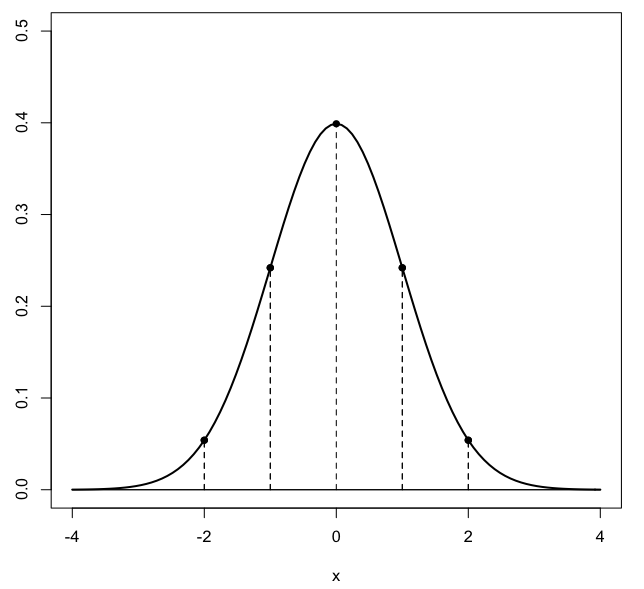
\includegraphics [scale=0.4] {gauss3.png} \end{center}
% \begin{bmatrix} a  &  b \\ c  &  d \end{bmatrix}
% \bigg |_

\Large
\noindent
We usually pick a coordinate system with axes perpendicular, scaled in the same units, with the label $x$ for horizontal and $y$ for vertical.  But for some problems, it can be useful to change the coordinate system.  There are a number of different possible ways to do this, as we'll see.  Importantly, there are some basic rules to follow to insure that the areas determined in the new coordinate system match up with those in the standard one.

Probably the simplest example of this is a linear stretching of one dimension, say, the $x$-axis.  Let's think about the problem of determining the area of the rectangle with one corner at $(0,0)$ and the other corner at $(2,1)$.  Although it seems like overkill, we're going to use (single variable) calculus to do it.  The upper edge is $y = f(x) = 1$.

\[ A = \int_{x=0}^{x=2} f(x)\ dx = \int_0^2 1\ dx = x  \ \bigg |_{0}^{2} = 2 \]

Seems to be correct.  :)
\vspace{5 px}
\noindent
Now, let us define a new variable $u$ which is exchanged at a rate of 2 $u$'s for every $x$.  (If $x=1$ then $u=2$, while if $x=2$ then $u=4$, and so on).
\[ u = 2x \]
We take the exact same shape, (with no change in the area), but change the horizontal coordinate system to be defined in terms of $u$.  The point $(2,1)$ becomes the point $(4,1)$ in the new coordinate system.  So we write
\[ A = \int_{u=0}^{u=4} f(u)\ du  \]
(This is wrong, but bear with me).  You see we have adjusted the limits of integration, since before we had the upper limit of $x=2$, now we have the upper limit of $u=4$.  That part is correct.  $f(x)$ is a constant, so everywhere $f(x) = f(u) = 1$ no matter the value of $x$ (or $u$).  Our mistake is that $du \neq dx$.
\[ du = 2\ dx \]
\[ \frac{1}{2} du = dx \]
so we substitute
\[ A = \int_{x=0}^{x=2} f(x)\ dx =  \int_{u=0}^{u=4} f(u)\ \frac{1}{2}du =  \frac{1}{2} \int_0^4 f(u)\ du = \frac{1}{2} \int_0^4 1\ du =  \frac{1}{2} \times 4 = 2 \]
which is correct.
We can do the very same problem in an even more complicated way, using multi-variable calculus.  Above, we imagine that what we are doing is slicing the area vertically into many slices with tiny width $dx$ and height $f(x)$ and adding all these together.  We can also imagine that we divide the area up into many little boxes of $dA$ and do the summation this way:
\[ A = \iint\limits_{R} 1 \ dA \]
The little boxes of area $dA$ have width $dx$ and height $dy$.
\[ A = \iint\limits_{R} 1 \ dA =   \int_{y=0}^{y=1} \int_{x=0}^{x=2} 1 \ dx \ dy  \]
We evaluate the \emph{inner} integral first, \emph{keeping $y$ constant}.
\[ = \int_{y=0}^{y=1}  x  \ \bigg |_{0}^{2} \ \ \ dy  \]
\[ = \int_{y=0}^{y=1}  2 \ dy  = 2y   \ \bigg |_{0}^{1} = 2  \]
(The real advantage of this is that we can substitute another function for $f(x,y) = 1$---see the Center of Mass write-up).  I introduce the two variable method as a way of approaching the next two problems.

\subsection*{Ellipse}

Let's think about a standard ellipse
\[ \frac{x^2}{a^2} + \frac{y^2}{b^2} = 1 \]
Following the example above, we could think about trying to compute the area of this ellipse as follows
\[ A = \iint\limits_{R} 1 \ dA = \iint\limits_{R} 1 \ dx \ dy \]
The problem is that we do not know how to specify the region, at least, not simply.  However, a little trick can make that problem go away!
\vspace{5 mm}

\noindent
We will change both the horizontal and vertical dimensions by a constant factor.  We compress (well, the opposite of stretching) $x$ by the factor $1/a$ and similarly compress $y$ by the factor $1/b$.  We make a change of variables
\[ x = au\] 
\[ y = bv \]
\[ dx = a\ du \]
\[ dy = b\ dv \]
So 
\[ dx \ dy = ab \ du \ dv \]
Substituting
\[ \frac{(au)^2}{a^2} + \frac{(bv)^2}{b^2} = u^2 + v^2 = 1\]
The substitution has converted the ellipse into a circle of radius $1$ and area $A = \pi$.
and
\[ A = \iint\limits_{R} 1 \ dx \ dy =  \iint\limits_{R} ab \ du \ dv = ab \iint\limits_{R} 1 \ du \ dv \]
Now, we know the area of the region in $u,v$ coordinates, it is a circle of radius $1$ and its area is just equal to $\pi$.  So finally
\[ A = ab \iint\limits_{R} 1 \ du \ dv = \pi a b \]
This is a really simple, beautiful result.  The two $r$'s in the formula $A= \pi r^2$ become $a \times b$.  Both dimensions make equivalent contributions to the area, as we'd expect.
\vspace{5 mm}

\noindent
The more formal way to do this is to compute what's called the Jacobian.  It gives the ratio between areas determined in two different coordinate systems.  We take the partial derivative of $x$ with respect to $u$ and $v$, and similarly for $y$.
\[ x_u = a \]
\[ x_v = 0 \]
\[ y_u = 0 \]
\[ y_v = b \]
The two partials ($x_v$ and $y_u$) are zero because $x$ does not depend on $v$ and  $y$ does not depend on $u$.

We evaluate the determinant of this matrix:
\[ J = 
\begin{vmatrix}
x_u & x_v \\
y_u & y_v 
\end{vmatrix} =
\begin{vmatrix}
a & 0 \\
0 & b
\end{vmatrix} =ab
\]
And that's the factor for converting between the two coordinate systems.
Sometimes the Jacobian is written as
\[ J = 
\begin{vmatrix}
x_u & y_u \\
x_v & y_v 
\end{vmatrix}
\]
but this doesn't change anything, because $det(A) = det(A^T)$.

To summarize:
\[ dx \ dy = J \ du \ dv \]
where
$J$ is computed as described.

\subsection*{Circle}

Another simple example is to find the area of a circle of radius $a$.  In terms of $x$ and $y$ we had previously
\[  \iint\limits_{R}  \ dA = \int_{x=0}^{x=a} \int_{y=0}^{y=\sqrt{a^2-x^2}} \ dy \ dx = \int_{x=0}^{x=a} \sqrt{a^2-x^2}  \ dx \]
This integral can be computed by doing a trig substitution, but there is an easier way, and that is to change to polar coordinates.  A naive attempt is
\[  \iint\limits_{R}  \ dA = \int_{\theta=0}^{\theta=2 \pi} \int_{r=0}^{r=a} \ dr \ d \theta = \int_{\theta=0}^{\theta=2 \pi} a \ d \theta = 2 \pi a \]
Obviously, this is wrong.
What happened is that the area element for a little bit of area $dA$ has an extra factor of $r$:

\[ dA = dx \ dy = r \ dr \ d \theta \]

\begin{center} 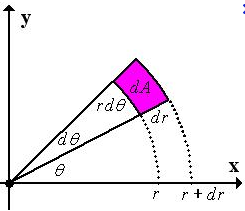
\includegraphics [scale=0.6] {polararea.png} \end{center}
As Strang says "areas always come from multiplying two lengths, and $d\theta$ is not a length."  He goes on to say that a wedge has area
\[ A = \frac{1}{2} r^2 \Delta \theta \]
The difference between wedges is $\Delta A$, and centering the change $\Delta r$ at $r$ we have:
\[ \Delta A = \frac{1}{2}(r + \frac{\Delta r}{2})^2 \Delta \theta - \frac{1}{2}(r - \frac{\Delta r}{2})^2 \Delta \theta \]
\[ = \frac{1}{2}(r^2 + r \Delta r + \frac{\Delta r^2}{4}) \Delta \theta - \frac{1}{2}(r^2 - r \Delta r + \frac{\Delta r^2}{4}) \Delta \theta \]
Neglecting the small term $\Delta r^2$:

\[ \Delta A =  r \Delta r \Delta \theta \]
The length of the curvy segment of arc depends on how far out we are on the radius.
\[ \iint\limits_{R}  \ dA = \int_{\theta=0}^{\theta=2 \pi} \int_{r=0}^{r=a} \ r \ dr \ d \theta = \int_{\theta=0}^{\theta=2 \pi} \frac{1}{2}a^2 \ d \theta = \pi a^2 \]
The Jacobian is done like this: 
\[ x = r\ cos\ \theta, \ \ y = r\ sin\ \theta \]
For convenience I'll define
\[ x_r = \frac{\partial x}{\partial r} = cos \ \theta, \ \ x_{\theta} = \frac{\partial x}{\partial \theta} = -r \ sin \ \theta \]
and similarly for $y$.  Then
\[ J = 
\begin{vmatrix}
x_r & x_{\theta} \\
y_r & y_{\theta} 
\end{vmatrix} =
\begin{vmatrix}
\cos\ \theta & -r \ sin\ \theta \\
\sin\ \theta & r \ cos\ \theta 
\end{vmatrix} = r (cos^2\ \theta + sin^2\ \theta) = r
\]
This is the factor for the ratio of areas under the two systems, and that's why we have $r\ dr \ d\theta$ in the integral.  Notice that when we took the partial derivatives, they were partials of $x,y$ with respect to $r,\theta$, and we end up multiplying $dr \ d\theta$ by J.

\subsection*{General method}

Suppose we wish to determine an area by integration and we're working with the unit square $x=0 \to x=1$ and $y=0 \to y=1$, sometimes written as $[\ 0,1\ ] \times [\ 0,1\ ]$.  The area is clearly just $1$.  Now we want to make a change of variables for some reason (to work on a function that's easier to deal with, or because we have some weird bounds in our problem).
\[ u = 3x-2y , \ \ v = x + y \]
We can figure out the "exchange rate" by tracing out the parallelogram formed by this linear transformation

\begin{align*}
& (0,0) \to (0,0) \\
& (0,1) \to (3,1) \\
& (1,1) \to (1,2) \\
& (0,1) \to (-2,1)
\end{align*}

If we think of the vectors $<3,1>$ and $<-2,1>$, the area of the parallelogram formed by these vectors is given by the determinant
\[
\begin{vmatrix}
3 & -2 \\
1 & \ \ 1 
\end{vmatrix} = 5
\]
The other way to do this calculation is (as we've been doing)
\[ u_x = 3 \]
\[ u_y = -2 \]
\[ v_x = 1 \]
\[ v_y = 1 \]
The Jacobian
\[ J = 
\begin{vmatrix}
u_x & u_y \\
v_x & v_y 
\end{vmatrix} = 
\begin{vmatrix}
3 & -2 \\
1 & \ \ 1 
\end{vmatrix}
= 3 - (-2) = 5 \]
Or more simply
\[ J = u_x v_y - u_y v_x = 3  - (-2) = 5 \]
And again, since we took the derivatives with respect to $x$ and $y$, we multiply $dx \ dy$ by $J$.

Each element of the area determined in $uv$ units is worth $5$ of an element in $xy$ units.
\[ 5 \iint\limits_{R}  f(x,y) \ dx \ dy = \iint\limits_{R}  f(u,v) \ du \ dv \]
\begin{equation}
\boxed{du \ dv = J \ dx \ dy }
\end{equation}
\vspace{5 mm}

\noindent
To say the above one more time in slightly different language, we have
\[ u = u(x,y) \]
\[ v = v(x,y) \]
If we change $x$ by a little bit $\Delta x$ and $y$ by a little bit $\Delta y$, by how much do $u$ and $v$ change? 
The linear approximation is
\[ \Delta u = u_x \Delta x + u_y \Delta y \]
\[ \Delta v = v_x \Delta x + v_y \Delta y \]
So for $\Delta x = 1$, the vector $<1,0>$ becomes
\[ \ <u_x ,v_x> \]
and $<0,1>$ becomes
\[ \ <u_y ,v_y> \]
and the area of the parallelogram formed by these two vectors (the area in $uv$-coordinates) is the absolute value of the cross product (think of them as lying in the plane, so there is only one term)
\[ <u_x ,v_x> \ \times  <u_y ,v_y > \]
\[ J = u_x v_y - u_y v_x \]
So for each unit $dx \ dy$ we get $du \ dv = J \ dx \ dy $ in the $uv$-coordinate system.

\subsection*{Tilted ellipse}
Here is the equation of an ellipse, although that may be hard to recognize at first.
\[ x^2 + 4xy + 13y^2 = 16 \]
If you remember (or look up) the formula
\[ Ax^2 + Bxy + Cy^2 + Dx + Ey + F = 0 \]
\[ A,B,C = 1,4,13 \]
The discriminant is
\[ B^2 - 4AC = 16 - 52 = -36 < 0 \]
Since it's $ < 0 $, this is an ellipse.  Or we could just get Grapher to plot it
\begin{center} 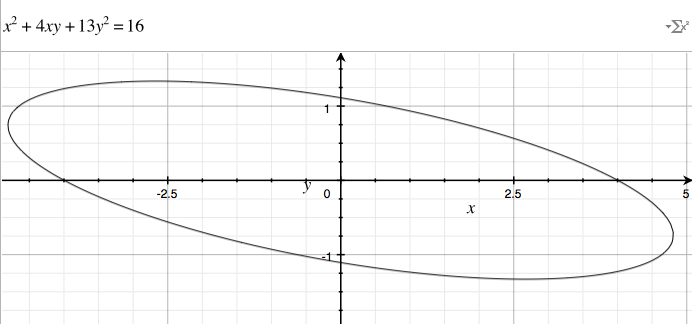
\includegraphics [scale=0.4] {tilted_ellipse.png} \end{center}
If we knew the angle, and there is a method for that, we could rotate to a new coordinate system and just compute the area as $\pi ab$.  However, there is another way which I think is easier.  We "complete the square" to remove the term which "mixes" $x$ and $y$.  Since
\[ (x + 2y)^2 = x^2 + 4xy + 4y^2 \]
Our equation is transformed as follows
\[ x^2 + 4xy + 13y^2 = 16 \]
\[ (x + 2y)^2 + 9y^2 = 16 \]
We do a substitution almost like before, but modified:
\[ u = x + 2y \]
\[ v = 3y \]
so now we have
\[ u^2 + v^2 = 16 \]
This is a circle of radius $4$ and area $16\pi$.
Now we just need the Jacobian:
\[ u_x = 1 \]
\[ u_y = 2 \]
\[ v_x = 0 \]
\[ v_y = 3 \]
\[ J = 
\begin{vmatrix}
u_x & u_y \\
v_x & v_y 
\end{vmatrix} = 
\begin{vmatrix}
1 & 2 \\
0 & 3 
\end{vmatrix}
= 3 \]
\[ du \ dv = 3 \ dx \ dy \]
When we took the partial derivatives, they were partials of $u,v$ with respect to $x,y$, so we end up multiplying $dx \ dy$ by J.
\[ \frac{1}{3} du \ dv = dx \ dy \]
We need to multiply the area by this factor to give a final answer of $16\pi/3$.

\subsection*{Varberg's example}
The next example is from Varberg, 17.16.
\begin{center} 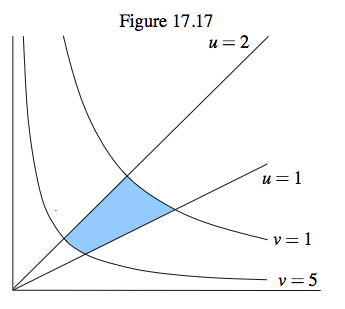
\includegraphics [scale=0.6] {Varberg-17-16.png} \end{center}
We have the lines $x=y$ and $x=2y$ and the curves $xy=1$ and $xy=5$.  Looks like $xy$ would be a good variable to have so
\[ u = \frac{x}{y} \]
\[ v = xy \]
These suggestions come from Varberg, not me.  :)  The boundaries of the region are just $u = 1 \rightarrow u = 2$ and $v = 1 \rightarrow v = 5 $.
Rearranging:
\[ x = uy \]
\[ x = \frac{v}{y} \]
\[ x^2 = xx = uy \ \frac{v}{y} =  uv \]

For the Jacobian, it is important to solve for $x,y$ in terms of $u,v$, and not the other way around, so that we'll have terms containing $u$ and $v$ in the final integral.
\[ x = \sqrt{uv} \]
\[ y^2 = \frac{x}{u} \frac{v}{x} = \frac{v}{u} \]
\[ y = \sqrt{\frac{v}{u}} \]
So 
\[ x_u = \frac{1}{2} \sqrt{\frac{v}{u}} \]
\[ x_v =  \frac{1}{2} \sqrt{\frac{u}{v}} \]
\[ y_u =  -\frac{1}{2u} \sqrt{\frac{v}{u}}\]
\[ y_v = \frac{1}{2} \sqrt{\frac{1}{uv}} \]
The Jacobian is then
\[ x_u y_v - x_v y_u \]
\[ \frac{1}{2} \sqrt{\frac{v}{u}} \ \frac{1}{2} \sqrt{\frac{1}{uv}} + \frac{1}{2} \sqrt{\frac{u}{v}} \  \frac{1}{2u} \sqrt{\frac{v}{u}} \]
\[ = \frac{1}{4u} + \frac{1}{4u} = \frac{1}{2u} \]
The area is 
\[ A = \iint\limits_{R} 1 \ dx \ dy =  \iint\limits_{R} \frac{1}{2u}  \ du \ dv \]
\[ = \int_{u=1}^{2} \ \int_{v=1}^{5} \frac{1}{2u}  \ dv \ du \]
\[ = 2 \int_{u=1}^{2} \ \frac{1}{u} \ du = 2 \ln 2 \]

\subsection*{Even weirder example from Auroux}

Suppose we have 
\[ \int_{y=0}^1 \int_{x=0}^1 x^2 y \ dx \ dy \]
For some strange reason we've decided that we're going to change to
\[ u = x, \ \ v = xy \]
\[ u_x = 1, \ \ u_y = 0, \ \ v_x = y, \ \ v_y = x \]
\[ J = 
\begin{vmatrix}
1 & 0 \\
y & x 
\end{vmatrix} = x \]

\[ du \ dv = x \ dx \ dy \]
\[ \iint\ xy \ x \ dx \ dy =  \iint\ v \ du \ dv  \]
That looks OK, but what are the limits?
\begin{center} 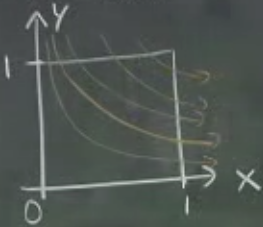
\includegraphics [scale=0.4] {changevar1.png} \end{center}
The first integral is with $v$ constant.  That means $xy=v$ is a constant, so we have different curves $xy = const$ (i.e. hyperobolas) between some limits.  The slices look like those in the figure above.

We enter our region from the top

\[ y= 1 \Longrightarrow u = x, v = xy = x = u \]
We leave the region on the side
\[ x= 1 \Longrightarrow u = 1 \]
\[ \int \int_{u=v}^{u=1} v \ du \ dv \]
The smallest value of $v$ is 
\[ x = 0 \Longrightarrow v = 0 \]
The largest value of $v$ is 
\[ x = 1, y = 1 \Longrightarrow v = 1 \]
\[ \int_{v=0}^{v=1} \int_{u=v}^{u=1} v \ du \ dv \]
The inner integral is 
\[ \int_{u=v}^{u=1} v \ du = uv \ \bigg |_{u=v}^{u=1} = v - v^2 \]
and the outer integral is
\[ \int_{v=0}^{v=1} v - v^2 \ dv = \frac{1}{2}v^2 - \frac{1}{3}v^3 \ \bigg |_{0}^{1} = \frac{1}{2} - \frac{1}{3} = \frac{1}{6} \]
We may have some doubt about the answer, so going back to what we started with and doing the integral we have
\[ \int_{y=0}^1 \int_{x=0}^1 x^2 y \ dx \ dy \]
The inner integral is 
\[ \int_{x=0}^1 x^2 y \ dx = \frac{1}{3}x^3y \ \bigg |_{0}^{1} = \frac{1}{3}y  \]
and the outer integral is
\[ \int_{y=0}^1  \frac{1}{3}y \ dy = \frac{1}{6}y^2 \ \bigg |_{0}^{1} = \frac{1}{6}  \]
which agrees.
\end{document}  